% tikzpic.teP
\documentclass[crop,tikz]{standalone}% 'crop' is the default for v1.0, before it was 'preview'

%Packages
\usepackage{xcolor}

%tikz libraries}}
\usetikzlibrary{shapes.geometric}

%Colors
\definecolor{recovery}{RGB}{27,158,119}
\definecolor{infection}{RGB}{217,95,2}
\definecolor{intervention}{RGB}{117,112,179}

% Formatting macros:
\tikzstyle{node}=[circle, draw]
\tikzstyle{edge}=[diamond, draw]

\tikzstyle{intervention}=[fill = intervention,text = white]
\tikzstyle{contact}=[fill = infection, text = white]
\tikzstyle{recovery}=[fill = recovery,text = white]


\begin{document}


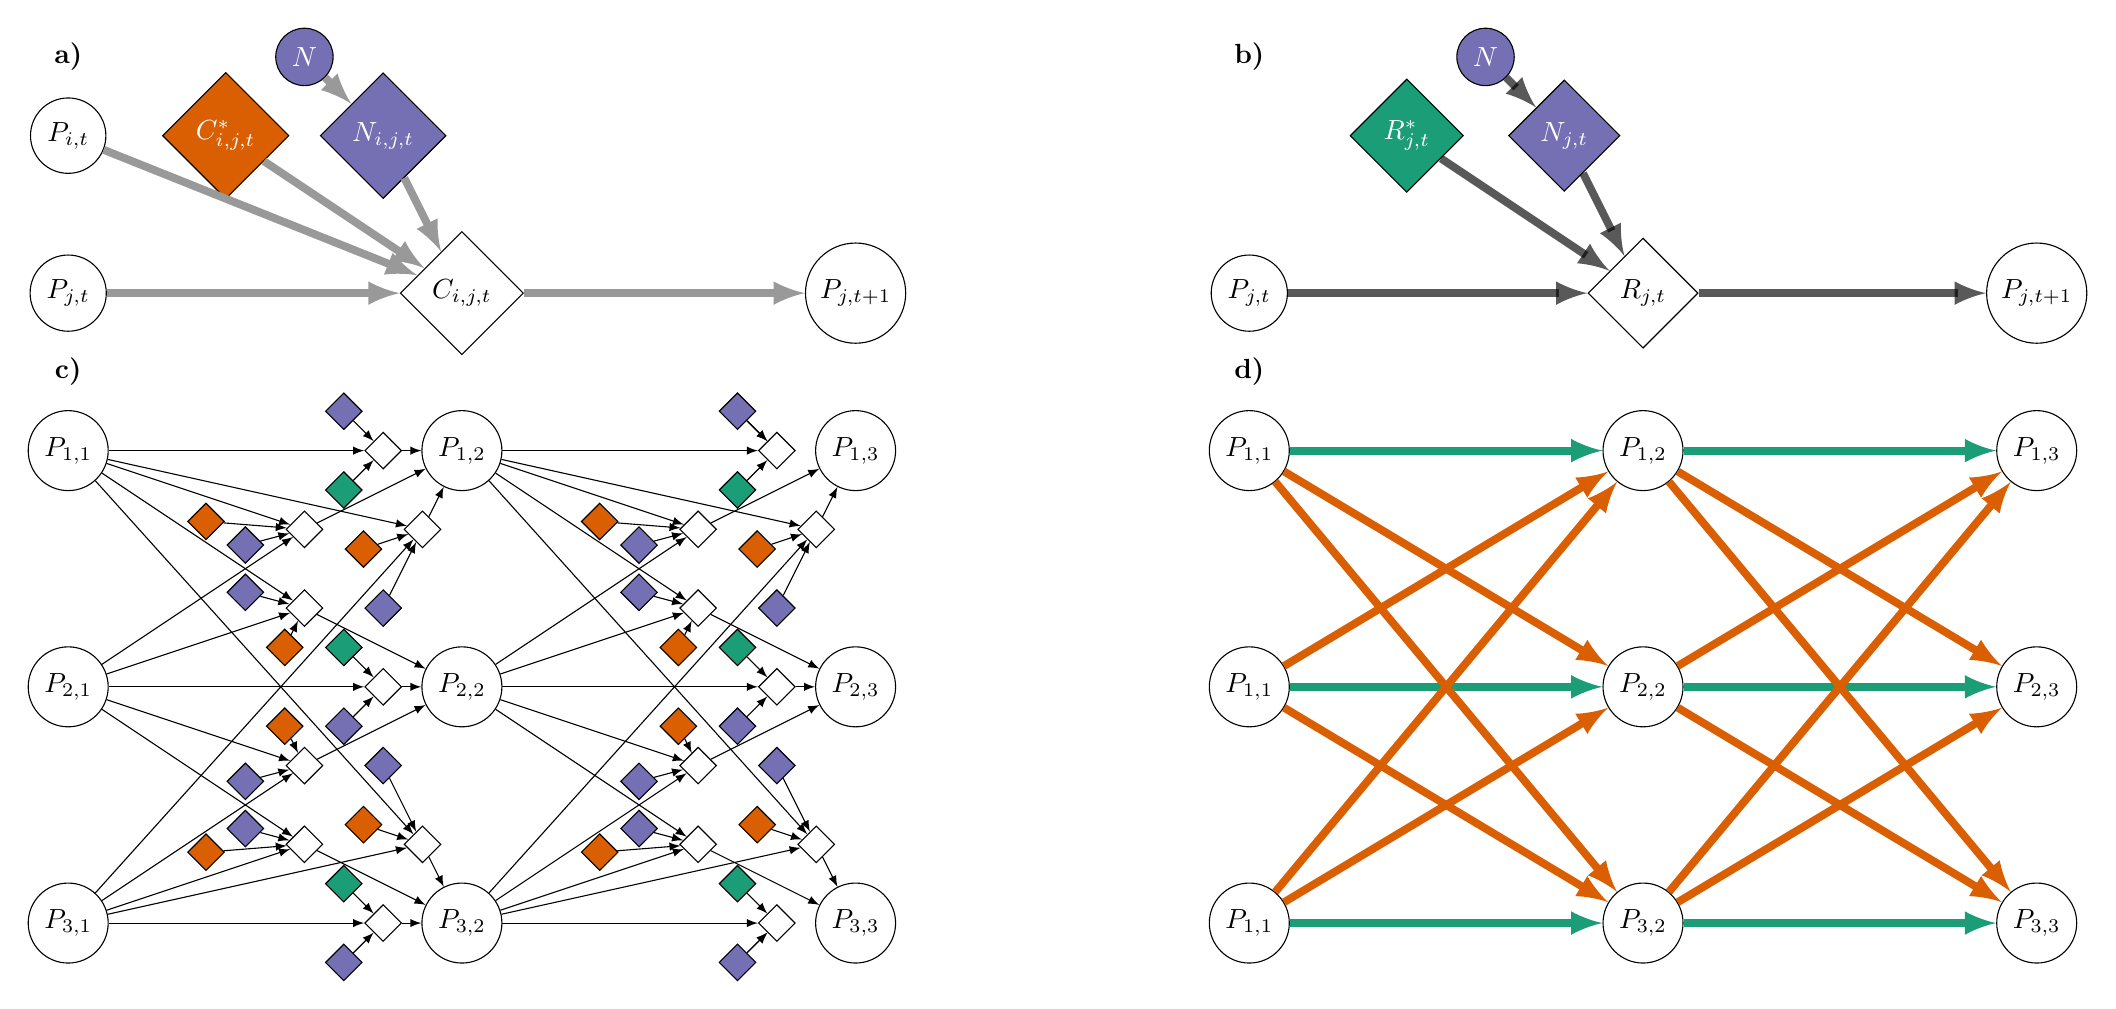
\begin{tikzpicture}
  %% Infectious Contacts
  \draw (-15,2) node[node] (P11) {$P_{i,t}$};
  \draw (-15,0) node[node] (P21) {$P_{j,t}$};
  \draw (-13,2) node[edge, contact] (E121) {$C^*_{i,j,t}$};
  \draw (-12,3) node[node,intervention] (I) {$N$};
  \draw (-11,2) node[edge, intervention] (I121) {$N_{i,j,t}$};
  \draw (-5,0) node[node] (P22) {$P_{j,t+1}$};
  \draw (-10,0) node[edge] (C121) {$C_{i,j,t}$};
  
  \draw[-latex,color=black!40!white,line width=1mm] (P11) -- (C121);
  \draw[-latex,color=black!40!white,line width=1mm] (P21) -- (C121);
  \draw[-latex,color=black!40!white,line width=1mm] (C121) -- (P22);
  \draw[-latex,color=black!40!white,line width=1mm] (E121) -- (C121);
  \draw[-latex,color=black!40!white,line width=1mm] (I121) -- (C121);
  \draw[-latex,color=black!40!white,line width=1mm] (I) -- (I121);
  
  
  %% Recovery
  \draw (0,0) node[node] (P21) {$P_{j,t}$};
  \draw (2,2) node[edge, recovery] (E121) {$R^*_{j,t}$};
  \draw (3,3) node[node, intervention] (I) {$N$};
  \draw (4,2) node[edge, intervention] (I11) {$N_{j,t}$};
  \draw (10,0) node[node] (P22) {$P_{j,t+1}$};
  \draw (5,0) node[ edge] (R121) {$R_{j,t}$};
  
  \draw[-latex,opacity=.65,line width=1mm] (P21) -- (R121);
  \draw[-latex,opacity=.65,line width=1mm] (R121) -- (P22);
  \draw[-latex,opacity=.65,line width=1mm] (E121) -- (R121);
  \draw[-latex,opacity=.65,line width=1mm] (I11) -- (R121);
  \draw[-latex,opacity=.65,line width=1mm] (I) -- (I11);
  
  
  %% Full
  \draw (-15,-5) node[node] (P11) {$P_{2,1}$};
  \draw (-15,-8) node[node] (P21) {$P_{3,1}$};
  \draw (-15,-2) node[node] (P31) {$P_{1,1}$};

  \draw (-10,-5) node[node] (P12) {$P_{2,2}$};
  \draw (-10,-8) node[node] (P22) {$P_{3,2}$};
  \draw (-10,-2) node[node] (P32) {$P_{1,2}$};

  \draw (-5,-5) node[node] (P13) {$P_{2,3}$};
  \draw (-5,-8) node[node] (P23) {$P_{3,3}$};
  \draw (-5,-2) node[node] (P33) {$P_{1,3}$};

  %%% Contact edges
  \draw (-11.25,-6.75) node[edge,contact] (E321) {};
  \draw (-11.25,-3.25) node[edge,contact] (E231) {};
  \draw (-10.5,-7) node[edge] (C321) {};
  \draw (-10.5,-3) node[ edge] (C231) {};
  \draw (-11,-6) node[edge,intervention] (I321) {};
  \draw (-11,-4) node[edge,intervention] (I231) {};

  \draw (-12.25,-4.5) node[edge,contact] (E311) {};
  \draw (-13.25,-2.9) node[edge,contact] (E131) {};
  \draw (-12,-4) node[edge] (C311) {};
  \draw (-12,-3) node[ edge] (C131) {};
  \draw (-12.75,-3.8) node[edge,intervention] (I311) {};
  \draw (-12.75,-3.2) node[edge,intervention] (I131) {};

  \draw (-13.25,-7.1) node[edge,contact] (E121) {};
  \draw (-12.25,-5.5) node[edge,contact] (E211) {};
  \draw (-12,-7) node[edge] (C121) {};
  \draw (-12,-6) node[ edge] (C211) {};
  \draw (-12.75,-6.8) node[edge,intervention] (I121) {};
  \draw (-12.75,-6.2) node[edge,intervention] (I211) {};
  
  \draw (-11.5,-2.5) node[edge,recovery] (E31) {};
  \draw (-11.5,-1.5) node[edge,intervention] (I31) {};
  \draw (-11,-2) node[edge] (R31) {};
  \draw (-11.5,-7.5) node[edge,recovery] (E21) {};
  \draw (-11.5,-8.5) node[edge,intervention] (I21) {};
  \draw (-11,-8) node[edge] (R21) {};
  \draw (-11.5,-4.5) node[edge,recovery] (E11) {};
  \draw (-11.5,-5.5) node[edge,intervention] (I11) {};
  \draw (-11,-5) node[edge] (R11) {};

  \draw (-6.25,-6.75) node[edge,contact] (E322) {};
  \draw (-6.25,-3.25) node[edge,contact] (E232) {};
  \draw (-5.5,-7) node[edge] (C322) {};
  \draw (-5.5,-3) node[ edge] (C232) {};
  \draw (-6,-6) node[edge,intervention] (I322) {};
  \draw (-6,-4) node[edge,intervention] (I232) {};

  \draw (-7.25,-4.5) node[edge,contact] (E312) {};
  \draw (-8.25,-2.9) node[edge,contact] (E132) {};
  \draw (-7,-4) node[edge] (C312) {};
  \draw (-7,-3) node[ edge] (C132) {};
  \draw (-7.75,-3.8) node[edge,intervention] (I312) {};
  \draw (-7.75,-3.2) node[edge,intervention] (I132) {};

  \draw (-8.25,-7.1) node[edge,contact] (E122) {};
  \draw (-7.25,-5.5) node[edge,contact] (E212) {};
  \draw (-7,-7) node[edge] (C122) {};
  \draw (-7,-6) node[ edge] (C212) {};
  \draw (-7.75,-6.8) node[edge,intervention] (I122) {};
  \draw (-7.75,-6.2) node[edge,intervention] (I212) {};
  
  \draw (-6.5,-2.5) node[edge,recovery] (E32) {};
  \draw (-6.5,-1.5) node[edge,intervention] (I32) {};
  \draw (-6,-2) node[edge] (R32) {};
  \draw (-6.5,-7.5) node[edge,recovery] (E22) {};
  \draw (-6.5,-8.5) node[edge,intervention] (I22) {};
  \draw (-6,-8) node[edge] (R22) {};
  \draw (-6.5,-4.5) node[edge,recovery] (E12) {};
  \draw (-6.5,-5.5) node[edge,intervention] (I12) {};
  \draw (-6,-5) node[edge] (R12) {};


  % \draw (-8.5,-5) node[edge,contact] (E132) {};
  % \draw (-8.5,-4) node[edge,contact] (E312) {};
  % \draw (-7,-5) node[ edge] (C132) {};
  % \draw (-7,-4) node[ edge] (C312) {};
  % \draw (-8,-4.75) node[edge,intervention] (I132) {};
  % \draw (-8,-4.25) node[edge,intervention] (I312) {};
  % 
  % \draw (-6.5,-8) node[edge,recovery] (E32) {};
  % \draw (-7,-7.75) node[edge,intervention] (I32) {};
  % \draw (-6,-7.5) node[edge] (R32) {};

  \draw[-latex] (P31) -- (C311);
  \draw[-latex] (P11) -- (C311);
  \draw[-latex] (E311) -- (C311);
  \draw[-latex] (I311) -- (C311);
  \draw[-latex] (C311) -- (P12);

  \draw[-latex] (P21) -- (C231);
  \draw[-latex] (P31) -- (C231);
  \draw[-latex] (E231) -- (C231);
  \draw[-latex] (I231) -- (C231);
  \draw[-latex] (C231) -- (P32);

  \draw[-latex] (P31) -- (C321);
  \draw[-latex] (P21) -- (C321);
  \draw[-latex] (E321) -- (C321);
  \draw[-latex] (I321) -- (C321);
  \draw[-latex] (C321) -- (P22);

  \draw[-latex] (P11) -- (C131);
  \draw[-latex] (P31) -- (C131);
  \draw[-latex] (E131) -- (C131);
  \draw[-latex] (I131) -- (C131);
  \draw[-latex] (C131) -- (P32);

  \draw[-latex] (P11) -- (C121);
  \draw[-latex] (P21) -- (C121);
  \draw[-latex] (E121) -- (C121);
  \draw[-latex] (I121) -- (C121);
  \draw[-latex] (C121) -- (P22);

  \draw[-latex] (P11) -- (C211);
  \draw[-latex] (P21) -- (C211);
  \draw[-latex] (E211) -- (C211);
  \draw[-latex] (I211) -- (C211);
  \draw[-latex] (C211) -- (P12);

  \draw[-latex] (P11) -- (R11);
  \draw[-latex] (P21) -- (R21);
  \draw[-latex] (P31) -- (R31);
  \draw[-latex] (E11) -- (R11);
  \draw[-latex] (E21) -- (R21);
  \draw[-latex] (E31) -- (R31);
  \draw[-latex] (I11) -- (R11);
  \draw[-latex] (I21) -- (R21);
  \draw[-latex] (I31) -- (R31);
  \draw[-latex] (R11) -- (P12);
  \draw[-latex] (R21) -- (P22);
  \draw[-latex] (R31) -- (P32);
  
  

  \draw[-latex] (P22) -- (C232);
  \draw[-latex] (P32) -- (C232);
  \draw[-latex] (E232) -- (C232);
  \draw[-latex] (I232) -- (C232);
  \draw[-latex] (C232) -- (P33);

  \draw[-latex] (P22) -- (C322);
  \draw[-latex] (P32) -- (C322);
  \draw[-latex] (E322) -- (C322);
  \draw[-latex] (I322) -- (C322);
  \draw[-latex] (C322) -- (P23);
  
  \draw[-latex] (P12) -- (C132);
  \draw[-latex] (P32) -- (C132);
  \draw[-latex] (E132) -- (C132);
  \draw[-latex] (I132) -- (C132);
  \draw[-latex] (C132) -- (P33);

  \draw[-latex] (P12) -- (C312);
  \draw[-latex] (P32) -- (C312);
  \draw[-latex] (E312) -- (C312);
  \draw[-latex] (I312) -- (C312);
  \draw[-latex] (C312) -- (P13);
  
  \draw[-latex] (P12) -- (C122);
  \draw[-latex] (P22) -- (C122);
  \draw[-latex] (E122) -- (C122);
  \draw[-latex] (I122) -- (C122);
  \draw[-latex] (C122) -- (P23);

  \draw[-latex] (P12) -- (C212);
  \draw[-latex] (P22) -- (C212);
  \draw[-latex] (E212) -- (C212);
  \draw[-latex] (I212) -- (C212);
  \draw[-latex] (C212) -- (P13);

  \draw[-latex] (P12) -- (R12);
  \draw[-latex] (P22) -- (R22);
  \draw[-latex] (P32) -- (R32);
  \draw[-latex] (E12) -- (R12);
  \draw[-latex] (E22) -- (R22);
  \draw[-latex] (E32) -- (R32);
  \draw[-latex] (I12) -- (R12);
  \draw[-latex] (I22) -- (R22);
  \draw[-latex] (I32) -- (R32);
  \draw[-latex] (R12) -- (P13);
  \draw[-latex] (I22) -- (R22);
  \draw[-latex] (I32) -- (R32);

  \draw (0,-2) node[node] (P11) {$P_{1,1}$};
  \draw (0,-5) node[node] (P21) {$P_{1,1}$};
  \draw (0,-8) node[node] (P31) {$P_{1,1}$};

  \draw (5,-2) node[node] (P12) {$P_{1,2}$};
  \draw (5,-5) node[node] (P22) {$P_{2,2}$};
  \draw (5,-8) node[node] (P32) {$P_{3,2}$};

  \draw (10,-2) node[node] (P13) {$P_{1,3}$};
  \draw (10,-5) node[node] (P23) {$P_{2,3}$};
  \draw (10,-8) node[node] (P33) {$P_{3,3}$};

  \draw[-latex,line width=1mm, color=recovery] (P11) -- (P12);
  \draw[-latex,line width=1mm, color=recovery] (P21) -- (P22);
  \draw[-latex,line width=1mm, color=recovery] (P31) -- (P32);
  \draw[-latex,line width=1mm, color=infection] (P11) -- (P22);
  \draw[-latex,line width=1mm, color=infection] (P21) -- (P12);
  \draw[-latex,line width=1mm, color=infection] (P11) -- (P32);
  \draw[-latex,line width=1mm, color=infection] (P21) -- (P32);
  \draw[-latex,line width=1mm, color=infection] (P31) -- (P12);
  \draw[-latex,line width=1mm, color=infection] (P31) -- (P22);

  \draw[-latex,line width=1mm, color=recovery] (P12) -- (P13);
  \draw[-latex,line width=1mm, color=recovery] (P22) -- (P23);
  \draw[-latex,line width=1mm, color=recovery] (P32) -- (P33);
  \draw[-latex,line width=1mm, color=infection] (P12) -- (P23);
  \draw[-latex,line width=1mm, color=infection] (P22) -- (P13);
  \draw[-latex,line width=1mm, color=infection] (P12) -- (P33);
  \draw[-latex,line width=1mm, color=infection] (P22) -- (P33);
  \draw[-latex,line width=1mm, color=infection] (P32) -- (P13);
  \draw[-latex,line width=1mm, color=infection] (P32) -- (P23);

  %% Caption thingies
  \draw (-15,3) node{\textbf{a)}};
  \draw (0,3) node{\textbf{b)}};
  \draw (-15,-1) node{\textbf{c)}};
  \draw (0,-1) node{\textbf{d)}};
\end{tikzpicture}


\end{document}
